\documentclass[a4paper,10pt]{article}

\usepackage[utf8]{inputenc}
% \usepackage[spanish]{babel}
\usepackage[dvips]{graphicx,color}
\usepackage{amsmath}
\usepackage{amssymb}
\usepackage{wrapfig}
\usepackage{bigints} % \int ===> \bigintssss, \bigintsss, \bigintss, \bigints, and \bigint
\usepackage{numprint} % para las cajas de las secciones de código
\usepackage[usenames,dvipsnames]{xcolor} % Texto con colores usando {\color{gray} XXXXX}
\usepackage{mathrsfs} % Para los simbolos del lagrangiano y el hamiltoniano
\usepackage{relsize} % Para hacer simbolos grandes \mathlarger y \mathsmaller
\usepackage{ifthen} % compilación condicional
\usepackage{alltt} % Entorno verbatim mejorado
\usepackage{setspace} % para cambiar el espaciado entre lineas
\usepackage{extarrows} % Para utilizar mas modelos de flechas ( sudo apt-get install texlive-math-extra )
\usepackage{listings} % Para escribir códigos

\setcounter{secnumdepth}{5} % Numeración de subsubsubsection = paragraph
\setcounter{tocdepth}{5} % Máxima profundidad en subsubsubsection = paragraph

\newboolean{englishVersion}
\setboolean{englishVersion}{true}

\voffset -2cm
\oddsidemargin 0.0cm
\evensidemargin -0.6cm
\textheight 23cm
\textwidth 16.5cm

% \decimalpoint

\def\bra#1{\mathinner{\langle{#1}|}}
\def\ket#1{\mathinner{|{#1}\rangle}}
\def\braket#1{\mathinner{\langle{#1}\rangle}}
\def\bbra#1{\bigl\langle#1\bigr|\,}
\def\kket#1{\,\bigl|#1\bigr\rangle}
\def\Bra#1{\left\langle#1\right|}
\def\Ket#1{\left|#1\right\rangle}
\def\BBra#1{\Bigl\langle#1\Bigr|\,}
\def\KKet#1{\,\Bigl|#1\Bigr\rangle}
\def\BBBra#1{\Biggl\langle#1\Biggr|\,}
\def\KKKet#1{\,\Biggl|#1\Biggr\rangle}
\def\wigner3j#1#2{ \left(\begin{array}{rrr} #1 \\ #2 \end{array}\right) }

\def\comb#1#2{\ensuremath{\left(\genfrac{}{}{0pt}{}{#1}{#2}\right)}}
\def\multiset#1#2{\ensuremath{\left(\kern-.3em\left(\genfrac{}{}{0pt}{}{#1}{#2}\right)\kern-.3em\right)}}

\newcommand{\tab}{\hspace{0.5cm}}
\newcommand{\n}{\\[1mm]}
\newcounter{cline}
\newcommand{\numc}{\stepcounter{cline}\npmakebox[2mm]{{\tiny \arabic{cline}}}\tab}
\newcommand{\numb}{\setcounter{cline}{0}}
\newcommand{\h}{\,\,\,}
\newcommand{\hh}{\,\,\,\,\,\,}
\newcommand{\RNum}[1]{{\small\uppercase\expandafter{\romannumeral #1\relax}}} % Numeros romanos por ejemplo \RNum{2}
\newcommand{\translation}[2]{\ifthenelse{\boolean{englishVersion}}{#1}{#2}}

%%%%%%%%%%%%%%%%%%%%%%%%%%%%%%%%%%%%%%%%%%%%%%%
% writing codes
%%%%%%%%%%%%%%%%%%%%%%%%%%%%%%%%%%%%%%%%%%%%%%%
% \definecolor{dkgreen}{rgb}{0,0.6,0}
% \definecolor{gray}{rgb}{0.5,0.5,0.5}
% \definecolor{mauve}{rgb}{0.58,0,0.82}
% 
% \lstset{frame=tb,
%   language=Java,
%   aboveskip=3mm,
%   belowskip=3mm,
%   showstringspaces=false,
%   columns=flexible,
%   basicstyle={\small\ttfamily},
%   numbers=none,
%   numberstyle=\tiny\color{gray},
%   keywordstyle=\color{blue},
%   commentstyle=\color{dkgreen},
%   stringstyle=\color{mauve},
%   breaklines=true,
%   breakatwhitespace=true,
%   tabsize=3
% }

\definecolor{mygreen}{rgb}{0,0.6,0}
\definecolor{mygray}{rgb}{0.5,0.5,0.5}
\definecolor{mymauve}{rgb}{0.58,0,0.82}

\lstset{ %
  backgroundcolor=\color{white},   % choose the background color; you must add \usepackage{color} or \usepackage{xcolor}
  basicstyle=\footnotesize,        % the size of the fonts that are used for the code
  breakatwhitespace=false,         % sets if automatic breaks should only happen at whitespace
  breaklines=true,                 % sets automatic line breaking
  captionpos=b,                    % sets the caption-position to bottom
  commentstyle=\color{mygreen},    % comment style
  deletekeywords={...},            % if you want to delete keywords from the given language
  escapeinside={\%*}{*)},          % if you want to add LaTeX within your code
  extendedchars=true,              % lets you use non-ASCII characters; for 8-bits encodings only, does not work with UTF-8
  frame=single,                    % adds a frame around the code
  keepspaces=true,                 % keeps spaces in text, useful for keeping indentation of code (possibly needs columns=flexible)
  keywordstyle=\color{blue},       % keyword style
  language=Fortran,                % the language of the code
  morekeywords={*,...},            % if you want to add more keywords to the set
  numbers=left,                    % where to put the line-numbers; possible values are (none, left, right)
  numbersep=10pt,                  % how far the line-numbers are from the code
  numberstyle=\tiny\color{mygray}, % the style that is used for the line-numbers
  rulecolor=\color{black},         % if not set, the frame-color may be changed on line-breaks within not-black text (e.g. comments (green here))
  showspaces=false,                % show spaces everywhere adding particular underscores; it overrides 'showstringspaces'
  showstringspaces=false,          % underline spaces within strings only
  showtabs=false,                  % show tabs within strings adding particular underscores
  stepnumber=1,                    % the step between two line-numbers. If it's 1, each line will be numbered
  stringstyle=\color{mymauve},     % string literal style
  tabsize=2,                       % sets default tabsize to 2 spaces
  title=\lstname                   % show the filename of files included with \lstinputlisting; also try caption instead of title
}
%%%%%%%%%%%%%%%%%%%%%%%%%%%%%%%%%%%%%%%%%%%%%%%

\translation{
\title{scift user manual}
}{
\title{scift manual de usuario}
}

\author{N.F. Aguirre}

\begin{document}

\maketitle

\tableofcontents

\label{capitulo FCINO}

\section{Introduction}

% Esta es la definición general de la FFT que habrá que definir en el futuro
% http://es.mathworks.com/help/symbolic/mupad_ref/ifourier.html

The continuous Fourier transform (CFT) of a function $f(t)$ and its inverse will be defined here as
\begin{equation}
\begin{gathered}
F(p) = \frac{1}{\sqrt{2\pi}}\int_{-\infty}^{\infty} f(x)\,\, e^{-ipx}\,dx
\\
f(x) = \frac{1}{\sqrt{2\pi}}\int_{-\infty}^{\infty} F(p)\,\, e^{ipx}\,dp
\end{gathered}
\end{equation}
where $i$ is the imaginary unit. The discrete Fourier Transform (DFT) and the inverse DFT of a
secuence $\mathbf{z}=\{z_1,z_2,\ldots,z_n\}$ (which may have real or complex values) will be defined as
\begin{equation}
\begin{gathered}
D_k(z) = \sum_{j=1}^n z_j e^{-2\pi i(j-1)(k-1)/n}\qquad\therefore\qquad k=1,2,\ldots,n
\\
D_k^{-1}(z) = \frac{1}{n}\sum_{j=1}^n z_j e^{2\pi i(j-1)(k-1)/n}\qquad\therefore\qquad k=1,2,\ldots,n
\end{gathered}
\end{equation}
An Fast Fourier Transform (FFT) computes the DFT and produces exactly the same result as evaluating the DFT definition directly; the most important difference 
is that an FFT is much faster.

Let us assume that $f(x)$ is a zero outside the interval $(-L/2,L/2)$. Let $\Delta x=L/n$ be the interval in $x$ for the $n$ input values of $f(x)$.

Further, Fourier transform software routines require a fixed discrete grid spacing.
Then the sampling interval on grid spacing is $\Delta x=a/n$, and $\Delta p =2\pi/(n\Delta x)$ on momentum spacing.
\begin{equation}
\begin{gathered}
x_j = j\Delta x, \qquad f_j = f(x_j) \qquad\therefore\qquad j=-\frac{n}{2},\ldots,\frac{n}{2}
\\[4mm]
p_k = k\Delta p, \qquad F_k = F(p_k) \qquad\therefore\qquad k=-\frac{n}{2},\ldots,\frac{n}{2}
\end{gathered}
\end{equation}
Then, we can write CFT as follows
\begin{equation}
F_k = \frac{\Delta x}{\sqrt{2\pi}}\sum_{j=-n/2}^{n/2} f_j\,\, e^{-2\pi i kj/n}
\qquad\therefore\qquad
k=-\frac{n}{2},\ldots,\frac{n}{2}
\label{eq: CFT raw}
\end{equation}
However most of implementations use positive indices, and therefore the spatial samples inside the sum must be re-arranged.
According with the FFTW library we use the standard order (\textit{s-order}) vector. This means that the
positive values are stored in the first half of the vector and the negative frequencies
are stored in backwards order in the second half of the vector, with the zero-value component
in the first element. We will represent this format as a \textit{tilde}, for example: $\mathbf{z}$
represent the array in \textit{s-order} and $\mathbf{\tilde{z}}$ in \textit{n-order}.
\begin{equation}
\text{$s$-order:}\qquad \boldsymbol{z} = \Bigl( z \Bigr)_{J=1}^n
\qquad\qquad\qquad\qquad\qquad\qquad
\text{$n$-order:}\qquad \tilde{\boldsymbol{z}} = \Bigl( z \Bigr)_{j=-n/2}^{n/2}
\end{equation}
where both sequences are related throught the following functions,
\begin{equation}
\tilde{\boldsymbol{z}} = \text{fftshift}(\boldsymbol{z}) \qquad\qquad \boldsymbol{z} = \text{ifftshift}(\tilde{\boldsymbol{z}})
\end{equation}
The next table represents the structure corresponds in the case where $n$ is an even number
\vspace{5mm}
\begin{center}
\begin{tabular}{c|rrrrrrrr}
$n$ & \multicolumn{4}{c|}{$n/2-1$} & \multicolumn{4}{c}{$n/2+1$}
\\\hline
$j$ & $-\frac{n}{2}+1$ & $-\frac{n}{2}+2$ & $\cdots$ & $-1$ &
$0$ & $\cdots$ & $\frac{n}{2}-1$ & $\frac{n}{2}$
\\
$J$ & $\frac{n}{2}+2$ & $\frac{n}{2}+3$ & $\ldots$ & $n$ &
$1$ & $\ldots$ & $\frac{n}{2}$ & 
$\frac{n}{2}+1$
\\\hline
\end{tabular}
\\[5mm]
\begin{tabular}{c|rrrrrrrr}
$n=8$& \multicolumn{3}{c|}{$3$} & \multicolumn{5}{c}{$5$}
\\\hline
$j$ & $-3$ & $-2$ & $-1$ & $0$ & $1$ & $2$ & $3$ & $4$
\\
$J$ & $6$ & $7$ & $8$ & $1$ & $2$ & $3$ & $4$ & $5$
\\\hline
\end{tabular}
\end{center}
If $n$ is odd then general structure of the table above still applies, but $n/2+1$ does not appear. 
\begin{center}
\begin{tabular}{c|rrrrrrrr}
$n$ & \multicolumn{4}{c|}{$\lfloor\frac{n}{2}\rfloor$} & \multicolumn{4}{c}{$\lfloor\frac{n}{2}\rfloor+1$}
\\\hline
$j$ & $-\lfloor\frac{n}{2}\rfloor$ & $-\lfloor\frac{n}{2}\rfloor+1$ & $\cdots$ & $-1$ &
$0$ & $\cdots$ & $\lfloor\frac{n}{2}\rfloor-1$ & 
$\lfloor\frac{n}{2}\rfloor$
\\
$J$ & $\lfloor\frac{n}{2}\rfloor+1$ & $\lfloor\frac{n}{2}\rfloor+2$ & $\ldots$ & $n$ &
$1$ & $\ldots$ & $\lfloor\frac{n}{2}\rfloor-1$ & 
$\lfloor\frac{n}{2}\rfloor$
\\\hline
\end{tabular}
\\[5mm]
\begin{tabular}{c|rrrrrrr}
$n=7$& \multicolumn{3}{c|}{$3$} & \multicolumn{4}{c}{$4$}
\\\hline
$j$ & $-3$ & $-2$ & $-1$ & $0$ & $1$ & $2$ & $3$
\\
$J$ & $5$ & $6$ & $7$ & $1$ & $2$ & $3$ & $4$
\\\hline
\end{tabular}
\end{center}
After this transformation Equation (\ref{eq: CFT raw}) can be reexpressed as follow
\begin{equation}
F_K = \frac{\Delta x}{\sqrt{2\pi}}\sum_{J=1}^{n} f_J\,\, e^{-2\pi i (K-1)(J-1)/n}
\qquad\therefore\qquad
K=1,2,\ldots,n
\label{eq: CFT end}
\end{equation}
The reordering of spatial samples means that the frequency samples should be re-arranged as well. 
Now it is clear that we can use the DFT definition to express the FT
(Denote K the new index in the frequency domain, which leads to the following expression:)
\begin{equation}
F_K = \frac{\Delta x}{\sqrt{2\pi}}D_K( \boldsymbol{f} )
\qquad\therefore\qquad
K=1,2,\ldots,n
\end{equation}



\clearpage
To be specific, the abscissas for the input data are,
\begin{equation}
x_j = \left(j-1-\frac{n}{2}\right)\Delta x \qquad\therefore\qquad j=1,2,\ldots,n
\end{equation}
The abscissas for the output data set will be defined as,
\begin{equation}
p_k = \left(k-1-\frac{n}{2}\right)\Delta p \qquad\therefore\qquad k=1,2,\ldots,n
\end{equation}
where $\Delta p = 2\pi/a = 2\pi/n\Delta x$ which conduce to the incertidumbre principle $\Delta x \Delta p = 2\pi/n$ and the important known as
``angular Nyquist frequency'' $\Omega=\pi/\Delta x$, which corresponds to the maximum and the negative mimimum value of frequency for the series.

% http://www.mvkonnik.info/2014/06/fft-ifft-and-why-do-we-need-fftshift.html
% Usually most of implementations uses positive indices, and therefore the spatial samples inside the sum must be rearranged:

\section{Convention}

To facilitate our discusion, we first define two general functions $f(x)$ and $F(p)$, which are
Fourier transforms of each other,
\begin{equation}
\begin{gathered}
\psi(x) = \frac{1}{\sqrt{2\pi\hbar}}\int_{-\infty}^{\infty} \psi(p)\,\, e^{ipx/\hbar}\,dp
\\
\psi(p) = \frac{1}{\sqrt{2\pi\hbar}}\int_{-\infty}^{\infty} \psi(x)\,\, e^{-ipx/\hbar}\,dx
\end{gathered}
\end{equation}
In general we are going to use atomic units ($\hbar=1$).

\begin{table}[h!]
\centering
\begin{tabular}{|c|c|}
\hline
\texttt{FFT}($\mathbf{f}$, $\tilde{\mathbf{F}}^\pm\rightarrow\mathbf{f}$, $\text{sign}=+1$) &
${\displaystyle
\tilde{F}_\alpha^\pm =
\frac{1}{\sqrt{2\pi}}\sum_{\beta=1}^{n} f_\beta\,\exp\left\{\pm 2\pi i\,\,\frac{(\alpha-1)(\beta-1)}{n}\right\}, \qquad \alpha = 1, 2, \ldots, n
}$
\\\hline
\texttt{iFFT}($\mathbf{\tilde{F}}$, $\mathbf{f}^\pm\rightarrow\mathbf{\tilde{F}}$, $\text{sign}=-1$) &
${\displaystyle
f_\beta =
\frac{1}{n\sqrt{2\pi}}\sum_{\alpha=1}^{n} \tilde{F}_\alpha^\pm\,\exp\left\{\mp 2\pi i\,\,\frac{(\beta-1)(\alpha-1)}{n}\right\}, \qquad \beta = 1, 2, \ldots, n
}$
\\\hline
\end{tabular}
\caption{\footnotesize{
asdasd
}}
\label{table: fft transforms}
\end{table}


% \translation{
\section{Fast Fourier transform (FFT)}

Let $\mathbf{f}=\{f_1,f_2,\ldots,f_n\}$ and $\mathbf{F}=\{F_1,F_2,\ldots,F_n\}$ two arrays of complex numbers.
The direct Discrete Fourier Transform (dDFT) of the array $\mathbf{f}$ is defined by the formula
\begin{equation}
F_\alpha^\pm = \sum_{\beta=1}^{n} f_\beta\,\exp\left\{\pm 2\pi i\,\,\frac{(\alpha-1)(\beta-1)}{n}\right\}, \qquad \alpha = 1, 2, \ldots, n
\end{equation}
The inverse DFT (iDFT) for the array $\mathbf{F}$ is defined as
\begin{equation}
f_\beta = \frac{1}{n}\sum_{\alpha=1}^{n} F_\alpha^\pm\,\exp\left\{\mp 2\pi i\,\,\frac{(\beta-1)(\alpha-1)}{n}\right\}, \qquad \beta = 1, 2, \ldots, n
\end{equation}
It differs from the direct transform by the normalization constant $1/n$.

The forward DFT (fDFT) corresponds to a sign of $+1$ in the exponent and backward DFT (bDFT) to a sign $-1$. Traditionally
the dDFT is associated with the sign $+$ and a the iDFT with the sign $-1$, in such case dDFT is equivalent to fDFT and
iDFT is equivalent to bDFT. However, here we will keep this difference.

According with the FFTW library we use the standard order (\textit{s-order}) output. This means that the
positive frequencies are stored in the first half of the output and the negative frequencies
are stored in backwards order in the second half of the output, with the zero-frequency component
in the first element. We will represent this format as a \textit{tilde}, for example: $\mathbf{x}$
represent the array in \textit{n-order} and $\mathbf{\tilde{x}}$ in \textit{s-order}.

There are three different ways to use the available methods available in scift
to calculate the FFT. 
\begin{equation}
\left[\mathbf{x},\mathbf{f}\right]
\mathrel{\substack{ \xrightarrow{\text{dFFT}(\pm)} \\ \xleftarrow{\text{iFFT}(\mp)} \\ . }}
\left[\boldsymbol{\tilde{\omega}},\mathbf{\tilde{F}}^\pm\right]
\mathrel{\substack{ \xrightarrow{\text{shift}} \\ \xleftarrow{\text{ishift}} \\ . }}
\left[\boldsymbol{\omega},\mathbf{F}^\pm\right]
\mathrel{\substack{ \xrightarrow{\text{dFFT}(\pm)} \\ \xleftarrow{\text{iFFT}(\mp)} \\ . }}
\left[\boldsymbol{\tilde{x}},\mathbf{\tilde{f}}^\pm\right]
\mathrel{\substack{ \xrightarrow{\text{shift}} \\ \xleftarrow{\text{ishift}} \\ . }}
\left[\boldsymbol{x},\mathbf{f}^\pm\right]
\end{equation}

\begin{equation}
\left[\mathbf{x},\mathbf{f}\right]
\longrightarrow
\left[\boldsymbol{\tilde{\omega}},\mathbf{\tilde{F}}\right]
\longrightarrow
\left[\boldsymbol{\omega},\mathbf{F}\right]
\end{equation}
When $n$ is even the location $n/2$ contains the most positive and negative frequencies
$\pm \frac{n/2}{nh}$ $\left( = \pm \frac{1}{2h} \right)$ which are equivalent.
This frequency is called Nyquist frequency. This is the highest frequency component that
should exist in the input series for the DFT to yield "uncorrupted" results. More
specifically if there are no frequencies above Nyquist the original signal can be exactly
reconstructed from the samples. 
\begin{center}
\begin{tabular}{|c|c|c|c|c|c|c|c|c|}
\multicolumn{5}{c|}{$n/2+1$} & \multicolumn{4}{c}{$n/2-1$} \\
\hline
$\tilde{\omega}_1$ & $\tilde{\omega}_2$ & $\tilde{\omega}_3$ & $\ldots$ & $\tilde{\omega}_{n/2+1}$ & $\tilde{\omega}_{n/2-1}$ & $\ldots$ & 
$\tilde{\omega}_{n-1}$ & $\tilde{\omega}_n$ \\
\hline\hline
$0$ & $\frac{1}{nh}$ & $\frac{2}{nh}$ & $\ldots$ & $\frac{n/2}{nh}$ & -$\frac{n/2-1}{nh}$ & $\ldots$ & $-\frac{2}{nh}$ & $-\frac{1}{nh}$ \\
\hline
\end{tabular}
\\[6mm]
\begin{tabular}{|c|c|c|c|c|c|c|c|c|}
\multicolumn{4}{c|}{$n/2-1$} & \multicolumn{5}{c}{$n/2+1$} \\
\hline
$\omega_1$ & $\ldots$ & $\omega_{n/2}$ & $\omega_{n/2+1}$ & $\omega_{n/2}$ & $\omega_{n/2+1}$ & $\omega_{n/2+2}$ & $\ldots$ & $\omega_n$ \\
\hline\hline
$\tilde{\omega}_{n/2+1}$ & $\ldots$ & $\tilde{\omega}_{n-1}$ & $\tilde{\omega}_{n}$ & $\tilde{\omega}_{1}$ & $\tilde{\omega}_{2}$ & $\tilde{\omega}_3$ & 
$\ldots$ & $\tilde{\omega}_{n/2}$ \\
\hline
-$\frac{n/2-1}{nh}$ & $\ldots$ & $-\frac{2}{nh}$ & $-\frac{1}{nh}$ & $0$ & $\frac{1}{nh}$ & $\frac{2}{nh}$ & $\ldots$ & $\frac{n/2}{nh}$ \\
\hline
\end{tabular}
\end{center}
\vspace{5mm}
If $n$ is odd then general structure of the table above still applies, but $n/2+1$ does not appear. 
\begin{center}
\begin{tabular}{|c|c|c|c|c|c|c|c|c|}
\multicolumn{5}{c|}{$n/2$} & \multicolumn{4}{c}{$n/2-1$} \\
\hline
$\tilde{\omega}_1$ & $\tilde{\omega}_2$ & $\tilde{\omega}_3$ & $\ldots$ & $\tilde{\omega}_{n/2}$ & $\tilde{\omega}_{n/2+1}$ & $\ldots$ & $\tilde{\omega}_{n-1}$ 
& $\tilde{\omega}_n$ \\
\hline\hline
$0$ & $\frac{1}{nh}$ & $\frac{2}{nh}$ & $\ldots$ & $\frac{n/2-1}{nh}$ & -$\frac{n/2-1}{nh}$ & $\ldots$ & $-\frac{2}{nh}$ & $-\frac{1}{nh}$ \\
\hline
\end{tabular}
\\[6mm]
\begin{tabular}{|c|c|c|c|c|c|c|c|c|}
\multicolumn{4}{c|}{$n/2-1$} & \multicolumn{5}{c}{$n/2$} \\
\hline
$\omega_1$ & $\ldots$ & $\omega_{n/2}$ & $\omega_{n/2+1}$ & $\omega_{n/2}$ & $\omega_{n/2+1}$ & $\omega_{n/2+2}$ & $\ldots$ & $\omega_n$ \\
\hline\hline
$\tilde{\omega}_{n/2+1}$ & $\ldots$ & $\tilde{\omega}_{n-1}$ & $\tilde{\omega}_{n}$ & $\tilde{\omega}_{1}$ & $\tilde{\omega}_{2}$ & $\tilde{\omega}_3$ & 
$\ldots$ & $\tilde{\omega}_{n/2}$ \\
\hline
-$\frac{n/2-1}{nh}$ & $\ldots$ & $-\frac{2}{nh}$ & $-\frac{1}{nh}$ & $0$ & $\frac{1}{nh}$ & $\frac{2}{nh}$ & $\ldots$ & $\frac{n/2-1}{nh}$ \\
\hline
\end{tabular}
\end{center}
\vspace{5mm}

% Given a window length n and a sample spacing d:
% 	!! @returns:	f : ndarray. Array of length n containing the sample frequencies.
% 	!! f = [0, 1, ...,   n/2-1,     -n/2, ..., -1] / (d*n)   if n is even
% 	!! f = [0, 1, ..., (n-1)/2, -(n-1)/2, ..., -1] / (d*n)   if n is odd

\subsection{Directly (High level interface)}
By using this option, scift internally make the shift and normalization for the $x$ coordinate.

\begin{equation}
\Bigl[x,f(x)\Bigr]
\stackrel{\text{5}}{\longrightarrow}
\Bigl[\omega,\hat{f}(\omega)\Bigr]
\end{equation}

\begin{equation}
\Bigl[\omega,\hat{f}(\omega)\Bigr]
\stackrel{\text{8}}{\longrightarrow}
\Bigl[x,f(x)\Bigr]
\end{equation}

\lstset{language=Fortran}
\begin{lstlisting}
call xGrid.init( -3.0_8*Math_PI, 3.0_8*Math_PI, 1000 )
call funcA.init( xGrid, funcTestWithNoise )
call funcA.save("func")  
  
funcA = FFT_fft( funcA )  
call funcA.save("Ffunc")  
  
funcA = FFT_ifft( funcA )  
call funcA.save("iFFfunc")  
\end{lstlisting}

This is the result

\begin{figure}[ht]
\centering
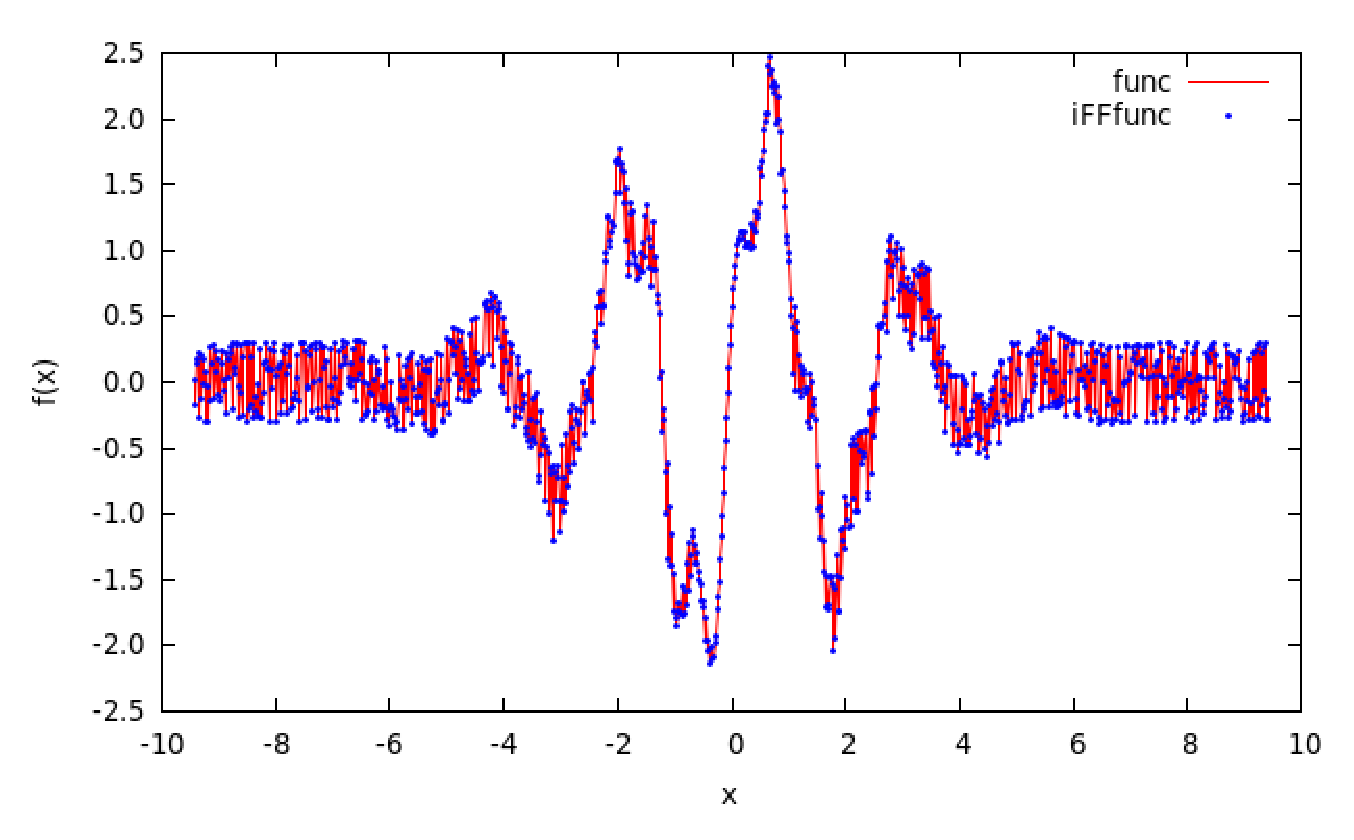
\includegraphics[scale=0.36]{images/FFT-func.eps}
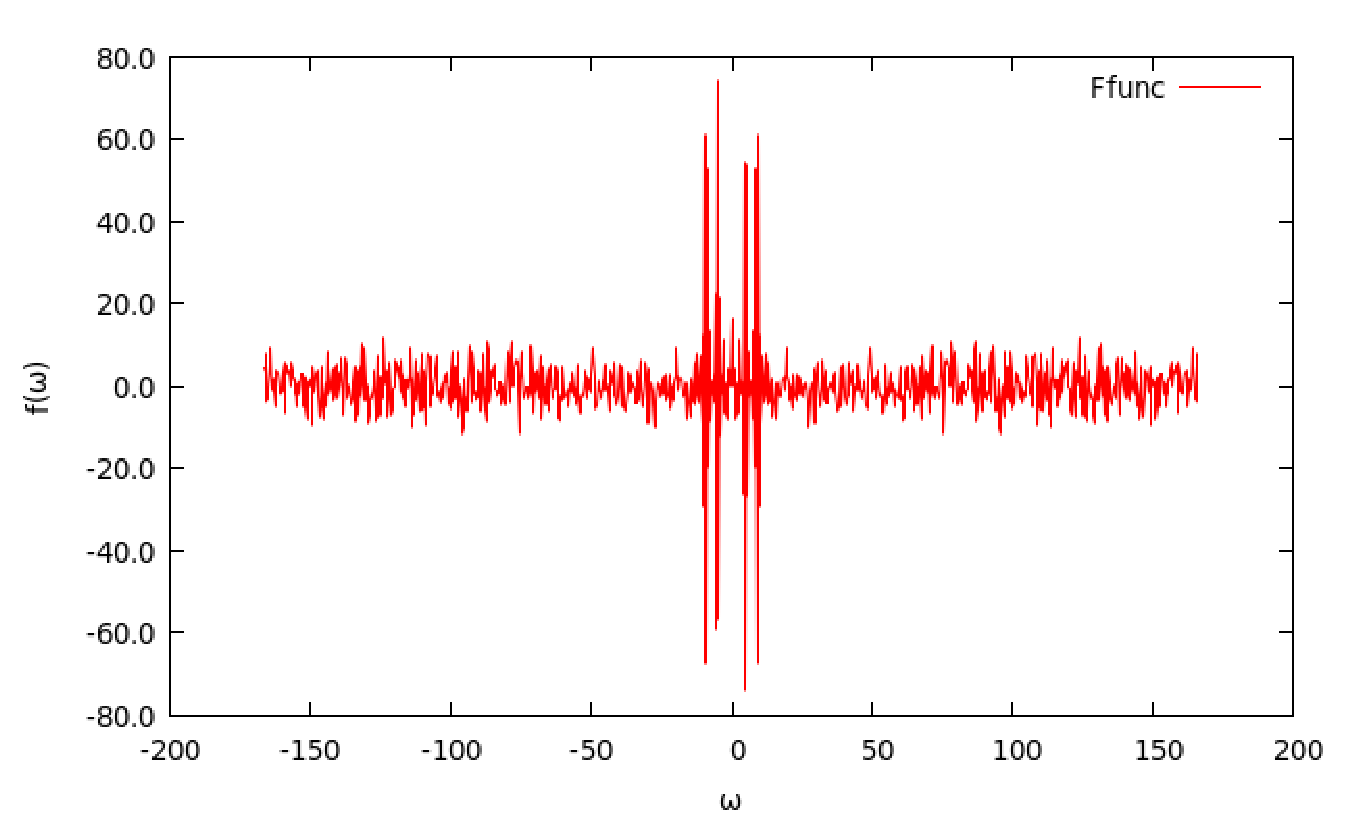
\includegraphics[scale=0.36]{images/FFT-Ffunc.eps}
\caption{\footnotesize{
Geometria para s=3
}}
% \label{}
\end{figure}

\subsection{By using plans (Low level interface)}
In this case is neccesary to keep in mind the reorganization on the frequency axis and the normalization
of the Fourier transform

\begin{equation}
\Bigl[x,f(x)\Bigr]
\stackrel{\text{8}}{\longrightarrow}
\Bigl[x,\hat{f}(\tilde{\omega})\Bigr]
\stackrel{\text{9}}{\longrightarrow}
\Bigl[\tilde{\omega},\hat{f}(\tilde{\omega})\Bigr]
\stackrel{\text{10}}{\longrightarrow}
\Bigl[\omega,\hat{f}(\omega)\Bigr]
\end{equation}

\begin{equation}
\Bigl[\omega,\hat{f}(\omega)\Bigr]
\stackrel{\text{13}}{\longrightarrow}
\Bigl[\tilde{\omega},\hat{f}(\tilde{\omega})\Bigr]
\stackrel{\text{14}}{\longrightarrow}
\Bigl[\tilde{\omega},F(x)\Bigr]
\stackrel{\text{15}}{\longrightarrow}
\Bigl[x,F(x)\Bigr]
\stackrel{\text{16}}{\longrightarrow}
\Bigl[x,f(x)\Bigr]
\end{equation}

\lstset{language=Fortran}
\begin{lstlisting}
call xGrid.init( -3.0_8*Math_PI, 3.0_8*Math_PI, 1000 )
call funcA.init( xGrid, funcTestWithNoise )
call funcA.save("func")
 		
planF = FFT_plan( funcA, FFT_FORWARD )
planB = FFT_plan( funcA, FFT_BACKWARD )
 		
call FFT_execute( planF )
funcA.xGrid = FFT_omegaGrid( funcA.xGrid )
call FFT_shift( funcA )
call funcA.save("Ffunc")

call FFT_ishift( funcA )
call FFT_execute( planB )
funcA.xGrid = FFT_xGrid( funcA.xGrid )
funcA = funcA/real( funcA.nPoints(), 8 )
call funcA.save("iFFfunc")

call FFT_destroyPlan( planF )
\end{lstlisting}

\subsection{By using the oriented object interface}
The function 
\begin{equation}
\begin{aligned}
&
\xlongleftrightarrow{\text{sync=F}\qquad\quad}
\quad\Bigl[x,\hat{f}(\tilde{\omega})\Bigr]
\\
\Bigl[x,f(x)\Bigr]\quad
&
\xlongleftrightarrow{\text{sync=T}\qquad\quad}
\quad\Bigl[\tilde{\omega},\hat{f}(\tilde{\omega})\Bigr]
\\
&
\xlongleftrightarrow{\text{sync=T,shift=T}}
\quad\Bigl[\omega,\hat{f}(\omega)\Bigr]
\end{aligned}
\end{equation}

\lstset{language=Fortran}
\begin{lstlisting}
call xGrid.init( -3.0_8*Math_PI, 3.0_8*Math_PI, 1000 )
call funcA.init( xGrid, funcTestWithNoise )
call funcA.save("func")  
  
call fft.init( funcA, FFT_SPATIAL_DOMAIN )

call fft.execute( FFT_FORWARD, sync=.true., shift=.true. )
call funcA.save("Ffunc")

call fft.execute( FFT_BACKWARD, sync=.true., shift=.true. )
call funcA.save("iFFfunc")
\end{lstlisting}

\subsection{Calculating the derivative of second order of a signal}
The function 
\begin{equation}
\frac{d^n}{dx^n}f(x) = (i\omega)^n\hat{f}(\omega)
\end{equation}

\begin{equation}
\Bigl[x,f(x)\Bigr]
\stackrel{\text{7}}{\longrightarrow}
\Bigl[x,\hat{f}(\tilde{\omega})\Bigr]
\xlongrightarrow{\text{9}}
\Bigl[x,(i\tilde{\omega})^2\hat{f}(\tilde{\omega})\Bigr]
\stackrel{\text{11}}{\longrightarrow}
\Bigl[x,\frac{d^2}{dx^2}f(x)\Bigr]
\end{equation}

\lstset{language=Fortran}
\begin{lstlisting}
call xGrid.init( -3.0_8*Math_PI, 3.0_8*Math_PI, 1000 )
call funcA.init( xGrid, funcTest )
call funcA.save("func")

call fft.init( funcA, FFT_SPATIAL_DOMAIN )

call fft.execute( FFT_FORWARD )

funcA.yArray = ( Math_I*fft.omega )**2*funcA.yArray

call fft.execute( FFT_BACKWARD )

call funcA.save("dfunc")

call funcB.init( xGrid, d2funcTest )
call funcB.save("exact")
\end{lstlisting}

This is the result

\begin{figure}[ht]
\centering
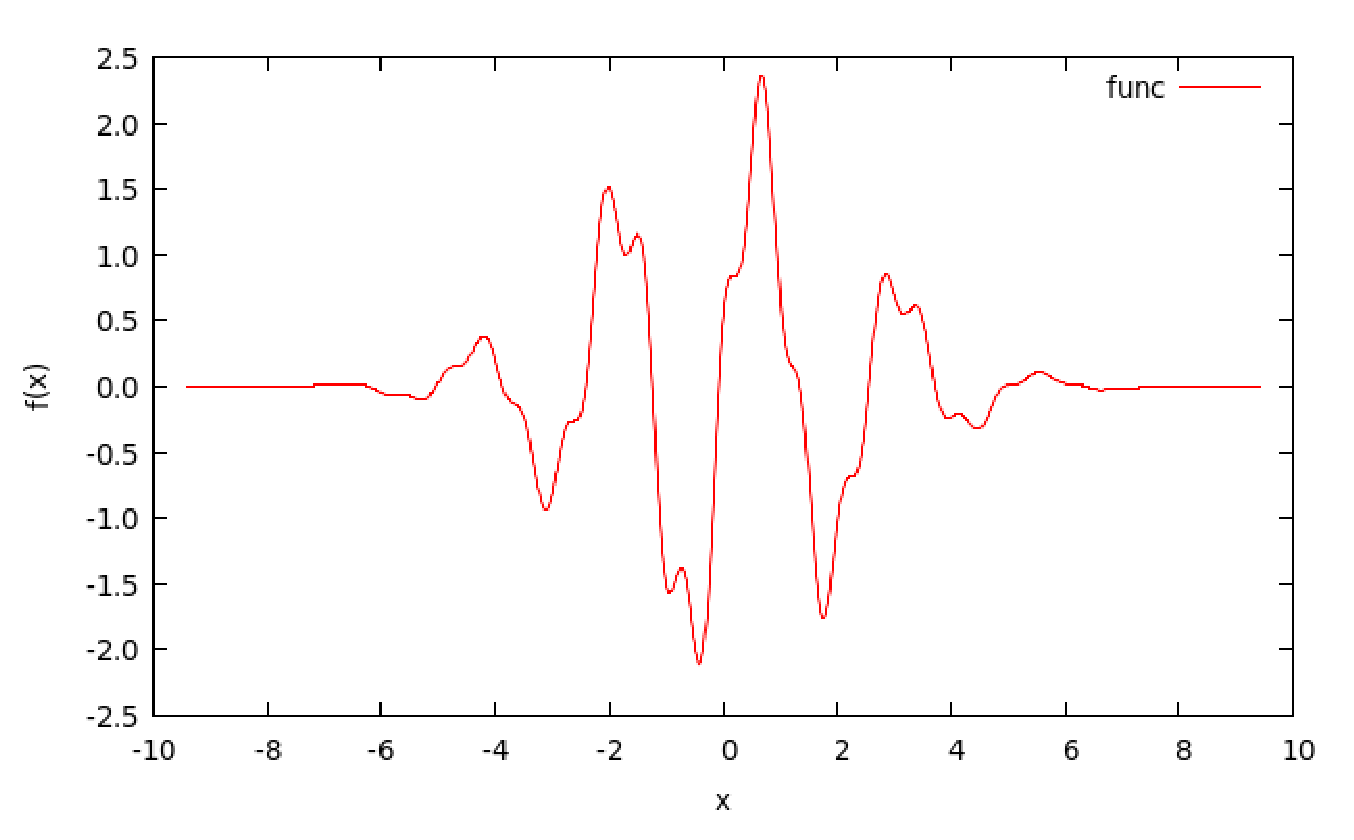
\includegraphics[scale=0.36]{images/FFT-func2.eps}
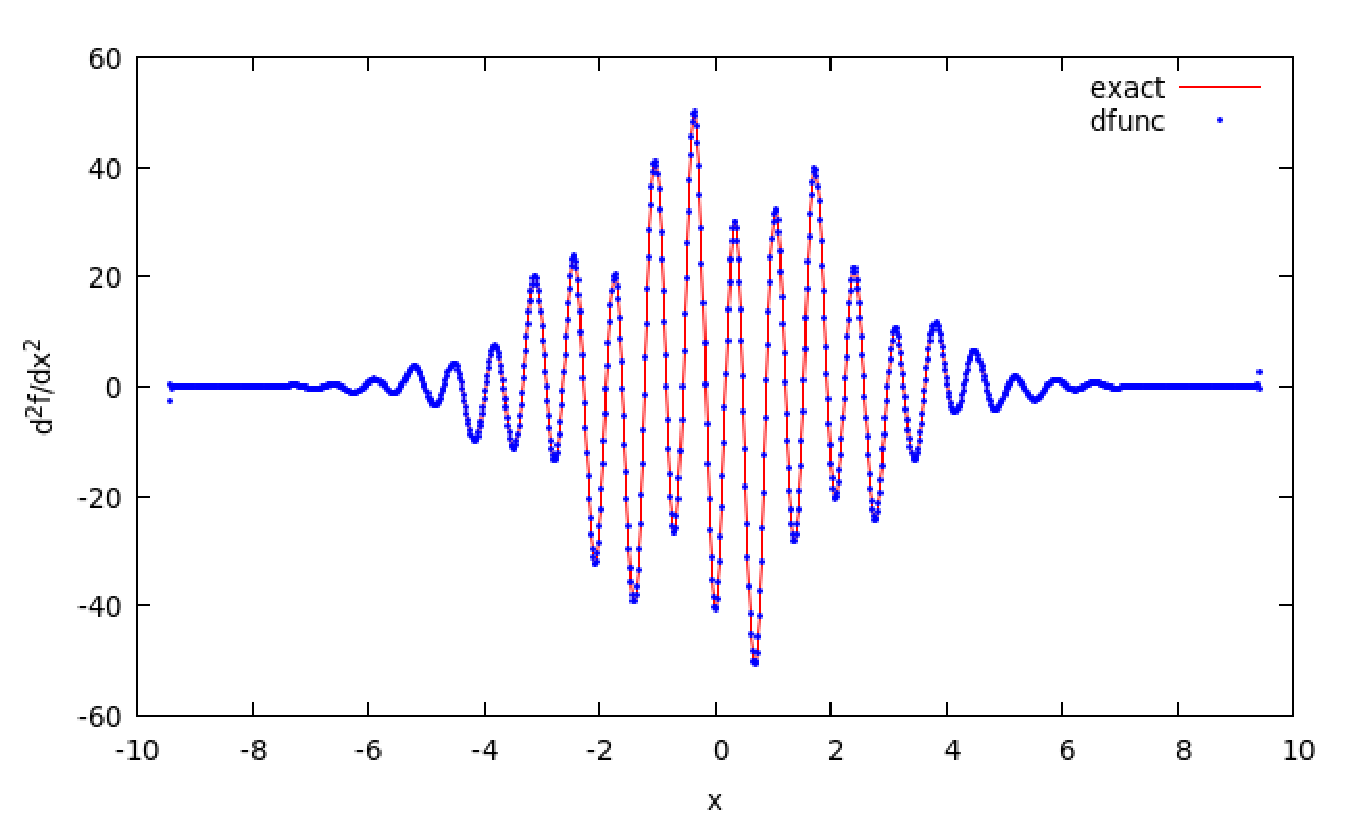
\includegraphics[scale=0.36]{images/FFT-dfunc.eps}
\caption{\footnotesize{
Left panel: Original function. Right panel: Derivative of second order of the signal calculated by using
the FFT interface, the exact solution is also included.
}}
% \label{}
\end{figure}


\end{document}
